\documentclass[tikz,border=8pt]{standalone}
\usepackage{amsmath,amssymb}
\usetikzlibrary{arrows.meta,calc,positioning,shapes.geometric}
\begin{document}
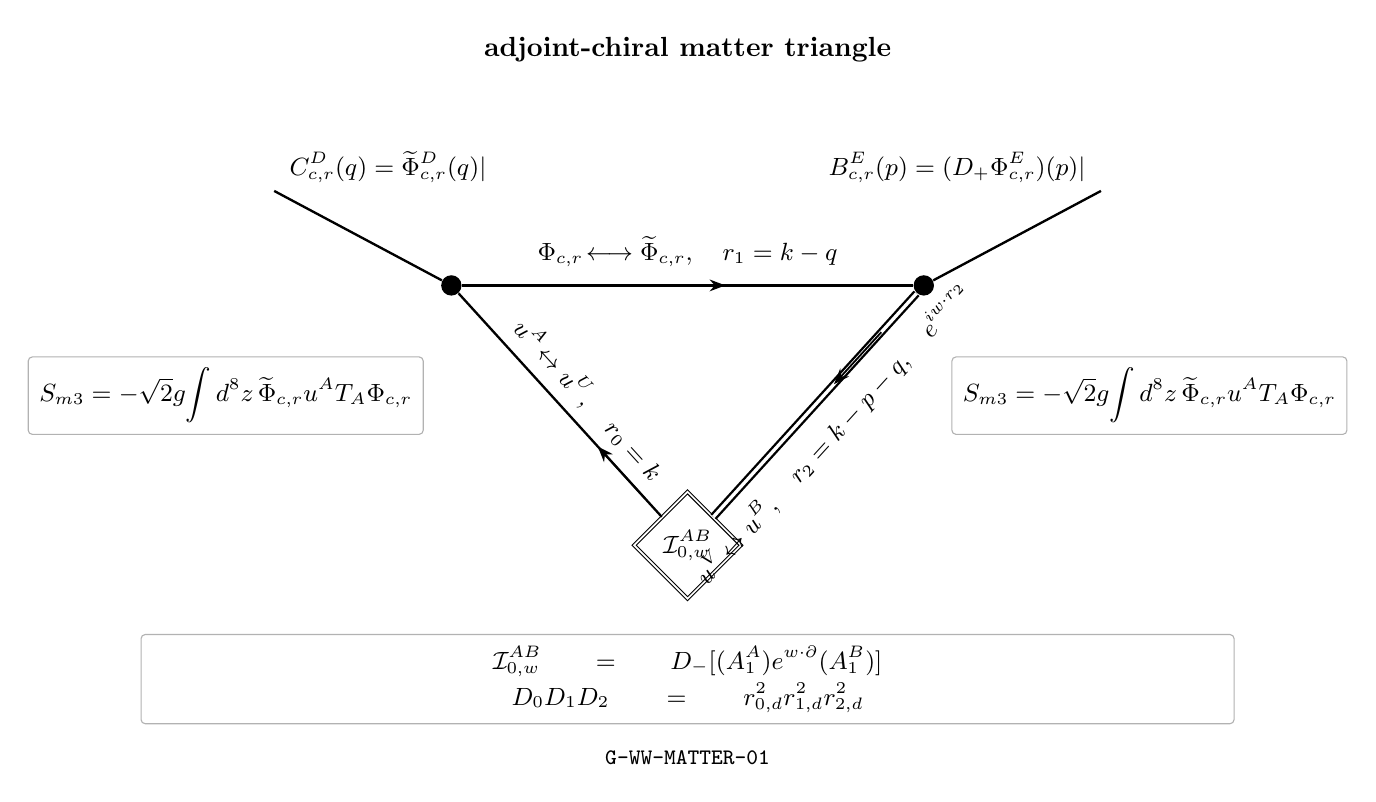
\begin{tikzpicture}[
  >=Stealth,
  momentum/.style={-{Stealth[length=2mm]},line width=0.65pt},
  propagator/.style={line width=0.85pt},
  insertion/.style={diamond,draw,double,inner sep=2.5pt,minimum size=10mm},
  action/.style={circle,fill=black,inner sep=2.6pt},
  formula/.style={draw=black!30,rounded corners=1.5pt,fill=white,inner sep=4pt,align=center},
  every node/.style={font=\small}
]
\node[font=\bfseries] at (0,4.55) {$\displaystyle \text{adjoint-chiral matter triangle}$};
\node[insertion] (I) at (0,-1.75) {$\displaystyle \mathcal I_{0,w}^{AB}$};
\node[action] (L) at (-3.0,1.55) {};
\node[action] (R) at (3.0,1.55) {};

\draw[propagator] (I) -- (L)
  node[pos=.45,sloped,above] {$\displaystyle u^A\!\leftrightarrow u^U,\quad r_0=k$};
\draw[propagator] (L) -- (R)
  node[midway,above=3pt] {$\displaystyle \Phi_{c,r}\!\longleftrightarrow\widetilde\Phi_{c,r},\quad r_1=k-q$};
\draw[propagator,double distance=1.2pt] (R) -- (I)
  node[pos=.53,sloped,below=3pt] {$\displaystyle u^V\!\leftrightarrow u^B,\quad r_2=k-p-q,\quad e^{iw\cdot r_2}$};

\draw[momentum] ($(I)!0.18!(L)$) -- ($(I)!0.38!(L)$);
\draw[momentum] ($(L)!0.38!(R)$) -- ($(L)!0.58!(R)$);
\draw[momentum] ($(R)!0.18!(I)$) -- ($(R)!0.38!(I)$);

\draw[propagator] (-5.25,2.75) -- (L)
  node[pos=.03,above right] {$\displaystyle C_{c,r}^D(q)=\widetilde\Phi_{c,r}^D(q)|$};
\draw[propagator] (R) -- (5.25,2.75)
  node[pos=.97,above left] {$\displaystyle B_{c,r}^E(p)=(D_+\Phi_{c,r}^E)(p)|$};

\node[formula,anchor=east] at (-3.35,.15)
  {$\displaystyle S_{m3}=-\sqrt2g\!\int d^8z\,\widetilde\Phi_{c,r}u^AT_A\Phi_{c,r}$};
\node[formula,anchor=west] at (3.35,.15)
  {$\displaystyle S_{m3}=-\sqrt2g\!\int d^8z\,\widetilde\Phi_{c,r}u^AT_A\Phi_{c,r}$};

\node[formula,text width=13.6cm] at (0,-3.45)
  {$\displaystyle \mathcal I_{0,w}^{AB}=D_-[(A_1^A)e^{w\cdot\partial}(A_1^B)]$\\[2pt]
   $\displaystyle D_0D_1D_2=r_{0,d}^2r_{1,d}^2r_{2,d}^2$};
\node[font=\ttfamily\footnotesize] at (0,-4.45) {G-WW-MATTER-01};
\end{tikzpicture}
\end{document}
